\documentclass[a4paper,12pt,twoside]{memoir}

% Castellano
\usepackage[spanish,es-tabla]{babel}
\selectlanguage{spanish}
\usepackage[utf8]{inputenc}
\usepackage[T1]{fontenc}
\usepackage{lmodern} % Scalable font
\usepackage{microtype}
\usepackage{placeins}

\RequirePackage{booktabs}
\RequirePackage[table]{xcolor}
\RequirePackage{xtab}
\RequirePackage{multirow}

% Links
\PassOptionsToPackage{hyphens}{url}\usepackage[colorlinks]{hyperref}
\hypersetup{
	allcolors = {red}
}

% Ecuaciones
\usepackage{amsmath}

% Rutas de fichero / paquete
\newcommand{\ruta}[1]{{\sffamily #1}}

% Párrafos
\nonzeroparskip

% Huérfanas y viudas
\widowpenalty100000
\clubpenalty100000

% Imagenes
\usepackage{graphicx}
\newcommand{\imagen}[2]{
	\begin{figure}[!h]
		\centering
		\includegraphics[width=0.9\textwidth]{#1}
		\caption{#2}\label{fig:#1}
	\end{figure}
	\FloatBarrier
}

\newcommand{\imagenflotante}[2]{
	\begin{figure}%[!h]
		\centering
		\includegraphics[width=0.9\textwidth]{#1}
		\caption{#2}\label{fig:#1}
	\end{figure}
}



% El comando \figura nos permite insertar figuras comodamente, y utilizando
% siempre el mismo formato. Los parametros son:
% 1 -> Porcentaje del ancho de página que ocupará la figura (de 0 a 1)
% 2 --> Fichero de la imagen
% 3 --> Texto a pie de imagen
% 4 --> Etiqueta (label) para referencias
% 5 --> Opciones que queramos pasarle al \includegraphics
% 6 --> Opciones de posicionamiento a pasarle a \begin{figure}
\newcommand{\figuraConPosicion}[6]{%
  \setlength{\anchoFloat}{#1\textwidth}%
  \addtolength{\anchoFloat}{-4\fboxsep}%
  \setlength{\anchoFigura}{\anchoFloat}%
  \begin{figure}[#6]
    \begin{center}%
      \Ovalbox{%
        \begin{minipage}{\anchoFloat}%
          \begin{center}%
            \includegraphics[width=\anchoFigura,#5]{#2}%
            \caption{#3}%
            \label{#4}%
          \end{center}%
        \end{minipage}
      }%
    \end{center}%
  \end{figure}%
}

%
% Comando para incluir imágenes en formato apaisado (sin marco).
\newcommand{\figuraApaisadaSinMarco}[5]{%
  \begin{figure}%
    \begin{center}%
    \includegraphics[angle=90,height=#1\textheight,#5]{#2}%
    \caption{#3}%
    \label{#4}%
    \end{center}%
  \end{figure}%
}
% Para las tablas
\newcommand{\otoprule}{\midrule [\heavyrulewidth]}
%
% Nuevo comando para tablas pequeñas (menos de una página).
\newcommand{\tablaSmall}[5]{%
 \begin{table}
  \begin{center}
   \rowcolors {2}{gray!35}{}
   \begin{tabular}{#2}
    \toprule
    #4
    \otoprule
    #5
    \bottomrule
   \end{tabular}
   \caption{#1}
   \label{tabla:#3}
  \end{center}
 \end{table}
}

%
% Nuevo comando para tablas pequeñas (menos de una página).
\newcommand{\tablaSmallSinColores}[5]{%
 \begin{table}[H]
  \begin{center}
   \begin{tabular}{#2}
    \toprule
    #4
    \otoprule
    #5
    \bottomrule
   \end{tabular}
   \caption{#1}
   \label{tabla:#3}
  \end{center}
 \end{table}
}

\newcommand{\tablaApaisadaSmall}[5]{%
\begin{landscape}
  \begin{table}
   \begin{center}
    \rowcolors {2}{gray!35}{}
    \begin{tabular}{#2}
     \toprule
     #4
     \otoprule
     #5
     \bottomrule
    \end{tabular}
    \caption{#1}
    \label{tabla:#3}
   \end{center}
  \end{table}
\end{landscape}
}

%
% Nuevo comando para tablas grandes con cabecera y filas alternas coloreadas en gris.
\newcommand{\tabla}[6]{%
  \begin{center}
    \tablefirsthead{
      \toprule
      #5
      \otoprule
    }
    \tablehead{
      \multicolumn{#3}{l}{\small\sl continúa desde la página anterior}\\
      \toprule
      #5
      \otoprule
    }
    \tabletail{
      \hline
      \multicolumn{#3}{r}{\small\sl continúa en la página siguiente}\\
    }
    \tablelasttail{
      \hline
    }
    \bottomcaption{#1}
    \rowcolors {2}{gray!35}{}
    \begin{xtabular}{#2}
      #6
      \bottomrule
    \end{xtabular}
    \label{tabla:#4}
  \end{center}
}

%
% Nuevo comando para tablas grandes con cabecera.
\newcommand{\tablaSinColores}[6]{%
  \begin{center}
    \tablefirsthead{
      \toprule
      #5
      \otoprule
    }
    \tablehead{
      \multicolumn{#3}{l}{\small\sl continúa desde la página anterior}\\
      \toprule
      #5
      \otoprule
    }
    \tabletail{
      \hline
      \multicolumn{#3}{r}{\small\sl continúa en la página siguiente}\\
    }
    \tablelasttail{
      \hline
    }
    \bottomcaption{#1}
    \begin{xtabular}{#2}
      #6
      \bottomrule
    \end{xtabular}
    \label{tabla:#4}
  \end{center}
}

%
% Nuevo comando para tablas grandes sin cabecera.
\newcommand{\tablaSinCabecera}[5]{%
  \begin{center}
    \tablefirsthead{
      \toprule
    }
    \tablehead{
      \multicolumn{#3}{l}{\small\sl continúa desde la página anterior}\\
      \hline
    }
    \tabletail{
      \hline
      \multicolumn{#3}{r}{\small\sl continúa en la página siguiente}\\
    }
    \tablelasttail{
      \hline
    }
    \bottomcaption{#1}
  \begin{xtabular}{#2}
    #5
   \bottomrule
  \end{xtabular}
  \label{tabla:#4}
  \end{center}
}



\definecolor{cgoLight}{HTML}{EEEEEE}
\definecolor{cgoExtralight}{HTML}{FFFFFF}

%
% Nuevo comando para tablas grandes sin cabecera.
\newcommand{\tablaSinCabeceraConBandas}[5]{%
  \begin{center}
    \tablefirsthead{
      \toprule
    }
    \tablehead{
      \multicolumn{#3}{l}{\small\sl continúa desde la página anterior}\\
      \hline
    }
    \tabletail{
      \hline
      \multicolumn{#3}{r}{\small\sl continúa en la página siguiente}\\
    }
    \tablelasttail{
      \hline
    }
    \bottomcaption{#1}
    \rowcolors[]{1}{cgoExtralight}{cgoLight}

  \begin{xtabular}{#2}
    #5
   \bottomrule
  \end{xtabular}
  \label{tabla:#4}
  \end{center}
}


















\graphicspath{ {./img/} }

% Capítulos
\chapterstyle{bianchi}
\newcommand{\capitulo}[2]{
	\setcounter{chapter}{#1}
	\setcounter{section}{0}
	\chapter*{#2}
	\addcontentsline{toc}{chapter}{#2}
	\markboth{#2}{#2}
}

% Apéndices
\renewcommand{\appendixname}{Apéndice}
\renewcommand*\cftappendixname{\appendixname}

\newcommand{\apendice}[1]{
	%\renewcommand{\thechapter}{A}
	\chapter{#1}
}

\renewcommand*\cftappendixname{\appendixname\ }

% Formato de portada
\makeatletter
\usepackage{xcolor}
\newcommand{\tutor}[1]{\def\@tutor{#1}}
\newcommand{\course}[1]{\def\@course{#1}}
\definecolor{cpardoBox}{HTML}{E6E6FF}
\def\maketitle{
  \null
  \thispagestyle{empty}
  % Cabecera ----------------
\noindent
\includegraphics[width=\textwidth]{cabecera}\vspace{1cm}%
  \vfill
  % Título proyecto y escudo informática ----------------
  \colorbox{cpardoBox}{%
    \begin{minipage}{.8\textwidth}
      \vspace{.5cm}\Large
      \begin{center}
      \textbf{TFG del Grado en Ingeniería Informática}\vspace{.6cm}\\
      \textbf{\LARGE\@title{}}
      \end{center}
      \vspace{.2cm}
    \end{minipage}

  }%
  \hfill\begin{minipage}{.20\textwidth}
    
\includegraphics[width=\textwidth]{escudoInfor}
  \end{minipage}
  \vfill
  % Datos de alumno, curso y tutores ------------------
  \begin{center}%
  {%
    \noindent\LARGE
    Presentado por \@author{}\\ 
    en Universidad de Burgos --- \@date{}\\
    Tutor: \@tutor{}\\
  }%
  \end{center}%
  \null
  \cleardoublepage
  }
\makeatother

\newcommand{\nombre}{Johnson Bolívar Arrobo Acaro} %%% cambio de comando

% Datos de portada
\title{Sistema clasificador de iris}
\author{Johnson Bolívar Arrobo Acaro}
\tutor{José Francisco Diez Pastor}
\date{\today}

\begin{document}

\maketitle


\newpage\null\thispagestyle{empty}\newpage


%%%%%%%%%%%%%%%%%%%%%%%%%%%%%%%%%%%%%%%%%%%%%%%%%%%%%%%%%%%%%%%%%%%%%%%%%%%%%%%%%%%%%%%%
\thispagestyle{empty}


\noindent
\includegraphics[width=\textwidth]{cabecera}\vspace{1cm}

\noindent D. José Francisco Diez Pastor, profesor del departamento de Ingeniería Informática, área de Lenguajes y Sistemas informáticos.

\noindent Expone:

\noindent Que el alumno D. \nombre, con DNI 71829434-C, ha realizado el Trabajo final de Grado en Ingeniería Informática titulado ``Sistema clasificador de iris''. 

\noindent Y que dicho trabajo ha sido realizado por el alumno bajo la dirección del que suscribe, en virtud de lo cual se autoriza su presentación y defensa.

\begin{center} %\large
En Burgos, {\large \today}
\end{center}

\vfill\vfill\vfill

% Author and supervisor
%\begin{minipage}{0.45\textwidth}
%\begin{flushleft} %\large
%Vº. Bº. del Tutor:\\[2cm]
%D. nombre tutor
%\end{flushleft}
%\end{minipage}
%\hfill
%\begin{minipage}{0.45\textwidth}
%\begin{flushleft} %\large
%Vº. Bº. del co-tutor:\\[2cm]
%D. nombre co-tutor
%\end{flushleft}
%\end{minipage}
%\hfill

%\vfill

% para casos con solo un tutor comentar lo anterior
% y descomentar lo siguiente
Vº. Bº. del Tutor:\\[2cm]
D. José Francisco Diez Pastor


\newpage\null\thispagestyle{empty}\newpage




\frontmatter

% Abstract en castellano
\renewcommand*\abstractname{Resumen}
\begin{abstract}
Los sistemas de seguridad basados en la biometría han experimentado una gran demanda y está presente cada vez más en productos cotidianos como \emph{smartphones} y \emph{tablets}.

En este trabajo se propone un sistema de identificación basado en el iris ocular, ya que se trata de un rasgo que proporciona una precisión muy alta y cuyas características se mantienen estables a lo largo de la vida.

Así mismo se ahondará en las técnicas existentes para llevar a cabo el proceso de identificación, desde los métodos convencionales usando algoritmos matemáticos hasta los métodos más actuales cómo el uso de Redes Neuronales, las cuales van ganando más popularidad debido a su facilidad de uso y los buenos resultados que arrojan.
\end{abstract}

\renewcommand*\abstractname{Descriptores}
\begin{abstract}
Biometría, iris, segmentación, sistemas de identificación, redes neuronales.
\end{abstract}

\clearpage

% Abstract en inglés
\renewcommand*\abstractname{Abstract}
\begin{abstract}
A \textbf{brief} presentation of the topic addressed in the project.
\end{abstract}

\renewcommand*\abstractname{Keywords}
\begin{abstract}
keywords separated by commas.
\end{abstract}

\clearpage

% Indices
\tableofcontents

\clearpage

\listoffigures

\clearpage

\listoftables
\clearpage

\mainmatter
\capitulo{1}{Introducción}

\epigraph{La probabilidad de que 2 iris cuenten con el mismo patrón es de aproximadamente 1 entre $10^{78}$. (La población mundial es de alrededor de $10^{10}$)}{Frankin Cheung}

La biometría se define cómo la toma de medidas estandarizadas de los seres vivos o de procesos biológicos \cite{intro:bio-wiki} que pueden ser usadas cómo medio para la identificación automática de individuos. 
Una buena biometría deberá ser:
\begin{itemize}
	\item \textbf{Universal:} cada individuo deberá tener unos determinados rasgos biométricos únicos.
	\item \textbf{Recolectable:} los rasgos biométricos podrán ser medidos y guardados.
	\item \textbf{Permanente:} no deberían variar a lo largo de la vida del individuo.
\end{itemize}
Los sistemas de reconocimiento basados en la biometría han experimentado un auge muy pronunciado en los últimos años, esto se puede ver reflejado en su implementación en dispositivos cotidianos del día a día, como \emph{smartphones} y \emph{tablets}.

Pero más allá de las huellas dactilares, la geometría de la mano o el reconocimiento facial (entre otros), existe otro rasgo físico nato que está cobrando mucha importancia, ya que comparado con los mencionados anteriormente, es mucho más seguro, se trata del iris ocular.

La idea de usar el iris para la identificación fue propuesto por el oftalmólogo Frank Burch en 1936, pero no fue hasta 1987 cuando Leonard Flon y Aran Safir patentaron la idea de Burch, aunque fueron incapaces de desarrollar por sí mismos los algoritmos necesarios, así que decidieron acudir a John Daugman, profesor en ese entonces de la Universidad de Harvard.
Los algoritmos desarrollados por Daugmann en 1994 son la base de todos los sistemas de reconocimiento de iris actuales~\cite{shiren:2009}.

El iris cómo rasgo biométrico aporta las siguientes ventajas~\cite{biometrics:2015}:
\begin{itemize}
	\item Es un rasgo que permanece invariable a lo largo de toda la vida del individuo y rara vez se ve afectado a causa de factores externos cómo accidentes o cirugías. Ver Figura \ref{fig:afghan-girl}
	\item Está constantemente protegido por la córnea
	\item Se trata de una técnica no invasiva, ya que no hace falta el contacto con el individuo para la toma de muestras, y por tanto su aceptabilidad por parte de estos es alta.
	\item Sus patrones son tan únicos que no existen 2 iris iguales, incluso los iris derecho e izquierdo del mismo individuo son distintos.
\end{itemize}

\imagen{afghan-girl}{Sharbat Gula, identificada 18 años mediante la aplicación de los algoritmos de Daugman.}

En el siguiente proyecto se expondrá el funcionamiento básico de un sistema de reconocimiento mediante el análisis de los patrones únicos del tejido membrano-muscular del iris mediante técnicas de \emph{Machine Learning}.

\section{Estructura de la memoria}\label{estructura-de-la-memoria}


La memoria sigue la siguiente estructura:
\begin{itemize}
\tightlist
\item
  \textbf{Introducción:} breve descripción del problema a resolver y la
  solución propuesta. Estructura de la memoria y listado de materiales
  adjuntos.
\item
  \textbf{Objetivos del proyecto:} exposición de los objetivos que
  persigue el proyecto.
\item
  \textbf{Conceptos teóricos:} breve explicación de los conceptos
  teóricos clave para la comprensión de la solución propuesta.
\item
  \textbf{Técnicas y herramientas:} listado de técnicas metodológicas y
  herramientas utilizadas para gestión y desarrollo del proyecto.
\item
  \textbf{Aspectos relevantes del desarrollo:} exposición de aspectos
  destacables que tuvieron lugar durante la realización del proyecto.
\item
  \textbf{Trabajos relacionados:} estado del arte en el campo del reconocimiento del iris.
\item
  \textbf{Conclusiones y líneas de trabajo futuras:} conclusiones
  obtenidas tras la realización del proyecto y posibilidades de mejora o
  expansión de la solución aportada.
\end{itemize}

\section{Materiales adjuntos}\label{materiales-adjuntos}
\begin{itemize}	
	\item \textbf{Anexos:}
	\begin{itemize}
	\tightlist
	\item
  		\textbf{Plan del proyecto software:} planificación temporal y estudio
  		de viabilidad del proyecto.
	\item
  		\textbf{Especificación de requisitos del software:} se describe la
  		fase de análisis; los objetivos generales, el catálogo de requisitos
  		del sistema y la especificación de requisitos funcionales y no
  		funcionales.
	\item
  		\textbf{Especificación de diseño:} se describe la fase de diseño; el
  		ámbito del software, el diseño de datos, el diseño procedimental y el
  		diseño arquitectónico.
	\item
  		\textbf{Manual del programador:} recoge los aspectos más relevantes
  		relacionados con el código fuente (estructura, compilación,
  		instalación, ejecución, pruebas, etc.).
	\item
  		\textbf{Manual de usuario:} guía de usuario para el correcto manejo 			de la aplicación.
	\end{itemize}
	
	\item \textbf{Notebooks de experimentación:} contienen todos los experimentos realizados y el conjunto de datasets empleados para la realización los mismos.
	\item \textbf{Aplicación de escritorio:} demo realizada en \emph{Tkinter} que muestra la funcionalidad del proyecto.
\end{itemize}

El proyecto, junto con los materiales mencionados están disponibles en el siguiente repositorio de GitHub: \url{https://github.com/jaa0124/iris_classifier}

\capitulo{2}{Objetivos del proyecto}

Este apartado explica de forma precisa y concisa cuales son los objetivos que se persiguen con la realización del proyecto. Se puede distinguir entre los objetivos marcados por los requisitos del software a construir y los objetivos de carácter técnico que plantea a la hora de llevar a la práctica el proyecto.

\capitulo{3}{Conceptos teóricos}

\section{Anatomía del iris}
El iris se corresponde con la parte coloreada del ojo, se trata de un músculo circular (o elíptico) protegido por la córnea en cuyo centro se encuentra la pupila. Consta de 2 músculos el \emph{dilatador} y el \emph{esfínter} cuya función es ajustar el tamaño del iris para controlar la cantidad de luz que entra en la pupila.
El conjunto iris-pupila se encuentra rodeado por una membrana de color blanco llamada \emph{esclera}. Ver Figura \ref{fig:eye-anatomy}

El color, la textura y los patrones del iris son únicos y se cree que se forman aleatoriamente durante el periodo embrionario (etapa comprendida entre fecundación y la octava semana de embarazo), de modo que incluso 2 gemelos genéticamente iguales tienen distintos patrones.

En un entorno con mucha luz el esfínter contrae la pupila, dejando pasar menos luz a la retina, mientras que en un entorno poco iluminado, el músculo dilatador, dilata la pupila para permitir la entrada de más luz.
El ojo está protegido externamente por los párpados y las pestañas, sin embargo suponen un problema ya que pueden ocultar significativamente el iris y por tanto resultar en un mal reconocimiento.
%\begin{figure}[h]
%  \centering
%    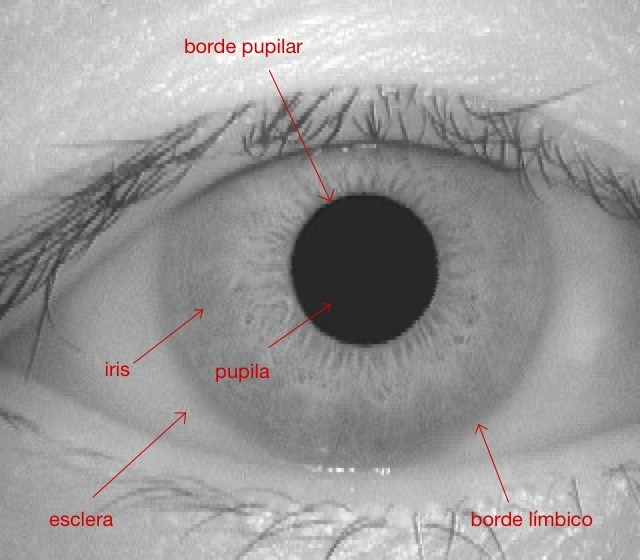
\includegraphics[width=0.7\textwidth]{eye-anatomy}
%  \caption{Imagen 001\_1\_1.bmp del dataset CASIA-Iris V1 que muestra las partes del ojo.}
%\end{figure}
%\newpage
\imagen{eye-anatomy}{Imagen 001\_1\_1.bmp del dataset CASIA-Iris V1 que muestra las partes del ojo.}

\section{Machine Learning}
El \emph{Machine Learning} es la rama de la Inteligencia Artificial que se encarga del desarrollo de técnicas que permitan extraer por sí mismos los patrones y relaciones existentes en los datos, es decir, su objetivo es conseguir que las máquinas aprendan sin necesidad de intervención humana ~\cite{wiki:2020,valdez:2018}.

A partir de unos datos de entrada (\emph{input/X}), y un resultado esperado para esos datos(\emph{outputs/y}), un algoritmo de \emph{Machine Learning} analizará las posibles relaciones entre estos y aprenderá de ellas (se entrenará) para realizar predicciones futuras.
\subsection{Tipos de Machine Learning}
\begin{itemize}
\tightlist
\item
  \textbf{Aprendizaje supervisado} este tipo de algoritmos generan una función que establece una relación entre los datos de entrada y las salidas deseadas (etiquetas/\emph{labels}).
  Existen 2 tipos:
  \begin{itemize}
      \item\textbf{Clasificadores: }clasifican los datos de entrada en grupos o clases. Existen 2 tipos de problemas de clasificación:
        \begin{itemize}
             \item\textbf{Binario: }existen únicamente 2 clases (0/1, \emph{true}/\emph{false}, o positivo/negativo)
              \item\textbf{Multiclase: }existen 3 o más clases.
        \end{itemize}
      \item\textbf{Regresores: }predicen un valor o cantidad.
  \end{itemize}
\item
  \textbf{Aprendizaje no supervisado} estos algoritmos sólo disponen de los datos de entrada, por lo que extraerán los patrones de los datos sin tener referencia alguna. Un ejemplo de este tipo de aprendizaje es el agrupamiento o \emph{clustering}
 \item
  \textbf{Aprendizaje por refuerzo} abarcan aquellos algoritmos que implementa un sistema de recompensas en función de las decisiones tomadas por un agente influenciado por el medio o entorno que le rodea.
\end{itemize}

En este proyecto se hará uso del \emph{Aprendizaje supervisado}, en el que tendremos como \emph{inputs} los atributos del iris, y cómo etiquetas, los nombres del individuo al que pertenecen dichos atributos.
Así mismo se planteará como un problema de clasificación multiclase en el que se cuenta concretamente con 108 clases que se corresponderan con los 108 individuos del dataset de CASIA V1 \ref{adquisicion_label}

Para la última fase del proceso del reconocimiento se usarán 4 clasificadores:
\begin{itemize}
\tightlist
    \item\textbf{Support Vector Machines }
    \item\textbf{Logistic Regression}
    \item\textbf{Nearest Neighbours} 
    \item\textbf{Random Forest}
\end{itemize}

\section{Deep Learning} \label{deep_learning}
Las algoritmos de \emph{Machine Learning} convencionales están limitados por su capacidad para procesar los datos de entrada.

Como alternativa surge el llamado \emph{Deep Learning} el cual permite desarrollar modelos computacionales compuestos internamente por múltiples capas de procesamiento.

\imagen{nn}{Red Neuronal ~\cite{sunil:2020}}

A la primera capa de la red se la denomina \emph{capa de entrada} y contiene las variables de entrada, le siguen una serie de capas intermedias denominadas \emph{capas ocultas}, donde las neuronas que se encuentren en la misma capa, recibiran la información procesada por la capa anterior y los cálculos que realice en dicha capa los pasará a la siguiente.
Finalmente está la \emph{capa de salida} que nos proporcionará el resultado de la red.

\section{Fases del reconocimiento}
Un sistema de reconocimiento tiene 3 fases:
\begin{enumerate}
	\item Adquisición de imágenes.
	\item Preprocesamiento de las imágenes:
	
	La cual se divide en 3 subfases:
	\begin{enumerate}
		\item Segmentación.
		\item Normalización.
		\item Extracción de atributos/\emph{features} (patrones del iris)
	\end{enumerate}
	\item Clasificación de las imágenes.

\end{enumerate}

\section{Adquisición de imágenes} \label{adquisicion_label}
Es la primera de todas las fases y también la más trascendental ya que es necesario que las muestras tengan la calidad necesaria para que la posterior extracción de patrones sea eficiente.

Las muestras de un iris se toman con cámaras desarrolladas específicamente para este propósito si bien para este proyecto no se contaba con este hardware se podría haber optado por usar una cámara convencional ~\cite{sanbishig:2017}, pero ello incluiría otro problema: conseguir muestras de un gran número de voluntarios.
Para evitarse los problemas mencionados se optó por usar un dataset de iris, concretamente el de CASIA en su versión 1 ~\cite{casia:1} el cual está disponible de forma gratuita mediante registro y autorización previa.

Este dataset cuenta con 756 imágenes del iris de 108 sujetos. La toma de muestras se realizó en 2 sesiones, tomándose 3 muestras en la primera sesión y 4 en la segunda, de modo que se cuenta con un total de 7 muestras por sujeto.
Cada muestra está en formato \emph{.bmp} y tienen una resolución de 320x280.
Para la toma de muestras usaron una cámara desarrollada por la propia CASIA.
\imagen{casia-camera}{Toma de muestras para el dataset CASIA-Iris-V1}
Con el objetivo de facilitar la detección de los bordes del iris, las muestras se han editado, de modo que se han eliminado los reflejos especulares~\footnote{Son las regiones más brillantes de la muestra del ojo, es decir, aquellos pixeles con valores iguales a 0. La superficie reflectante de la córnea y la fuente de luz usada para tomar la muestra son la principal causa de la aparición de estos reflejos.}.

Cabe recalcar que dichas ediciones son mínimas y se aplican únicamente en la pupila ~\cite{kumar:2019}, la cual no proporciona ninguna información útil para las etapas posteriores de extracción y clasificación de los patrones del iris ~\cite{bowyer:2008}.
\imagen{specular}{Imagen S1143R01.jpg perteneciente CASIA-Interval-V3 con regiones especulares(izquierda). Imagen 001\_1\_1.bmp de CASIA-Iris-V1 sin regiones especulares(derecha)}

\section{Preprocesamiento} \label{prepro}
Como puede apreciarse en la figura de la derecha de la imagen ~\ref{fig:specular}, la muestra es del ojo completo, pero para el reconocimiento únicamnete nos interesa la región del iris, por lo que elementos como pestañas, párpados, esclera \emph{etc} han de eliminarse ya que no aportan nada.
Así mismo dependiendo de las condiciones en las que se tomaron las muestras es posible que el tamaño de los iris varíen debido a la dilatación o la contracción de la pupila.

Es por ellos que ha de procesarse la imagen para localizar y aislar el iris (\emph{segmentar}) y ajustarlo a un tamaño estándar (\emph{normalizar})


\subsection{Segmentación} \label{segmentacion}
En esta etapa se requiere detectar de manera automática los bordes \emph{límbico} y \emph{pupilar} del ojo aislando la región del iris y excluyendo el resto de la imagen, es decir, se busca el \emph{ROI (Region of interest)}

El iris se corresponde con la región circular comprendido entre la pupila y la esclera.
La mayoría de fallos en un sistema de reconocimiento de iris se debe a una segmentación deficiente de las imágenes, por lo que se han de tener en cuenta los siguientes factores:
\begin{itemize}
    \item El iris se encuentra obstruido por pestañas, párpados y reflejos especulares.
    \item Tanto iris como pupila no son siempre circulares sino que pueden tener forma elíptica, y su forma puede variar dependiendo de la forma en que se tome la muestra.
    \item Factores cómo muestras desenfocadas, con mucho ruido, poca calidad.. (estos han de tenerse en cuenta en la etapa de adquisición de imágenes)
\end{itemize}

\imagen{segmentado}{Detección incorrecta de los bordes límbico y pupilar (izquierda) y la correcta (derecha)}
Como se ha dicho anteriormente, los algoritmos de Daugman son la base de los sistemas de reconocimiento actuales, pero no son los únicos métodos existentes.

\begin{itemize}
    \item\textbf{Operador Integro-Diferencial de Daugman:} Daugman propuso el primer modelo funcional para un sistema de reconocimiento de iris y consiste en un detector de bordes circulares que busca el máximo valor del cambio de tonalidad en la imagen utilizando la integral de línea de varios círculos concéntricos.
    
    El operador viene determinado por la siguiente ecuación~\cite{kazakov:2011}:
    
    \emph{añdir refrencia iris detection and noramlization[4]}
    \begin{equation*}
    \max_{\substack(r,x_{0},y_{0})}\left | G_{\sigma }(r)*\frac{\partial }{\partial x}\oint_{(r,x_{0},y_{0})} \frac{I(x,y)}{2\pi r}ds \right |
    \end{equation*}
    donde la intendidad del pixel en las coordenadas $I(x,y)$ se corresponde con la imagen del ojo, $ds$ es el arco diferencial del círculo de radio $r$ y coordenadas $(x_{0},y_{0})$. $G_{\sigma}$
    es una función que suaviza la imagen como un filtro Gaussiano de tamaño $\sigma$. Dado que utiliza información derivativa de primer orden, se computa muy rápidamente ~\cite{yonekura:2014}.
    
    Lo que hace la ecuación es encontrar el máximo cambio entre las intensidades medias de dos circunferencias concéntricas consecutivas. En el borde entre el iris y la esclera este cambio será máximo porque la última circunferencia concéntrica del iris será oscura y la primera de la esclera será blanca. Dicho cambio viene dado con la derivada.
    
    La media de todos los píxeles de cada una de las posibles circunferencias concéntricas viene de la integral de la división entre la intensidad y $2 \pi r$ ya que esa es la longitud de la circunferencia.
    
    \item\textbf{Transformada de Hough:} parte de la idea de que los bordes límbico y pupilar pueden ser considerados como círculos, la Transformada de Hough original se usaba en un principio para la detección de líneas en una imagen, sin embargo más adelante se extendió para que pudiera reconocer también circulos y circunferencias, pasó a denominarse \emph{Transformada de Hough Circular}.
    
    Su funcionamiento es el siguiente:
    Primero se realzan los bordes para generar el \emph{edge map} de la imagen mediante el cálculo de la primera derivada de las intensidades de los píxeles y a continuación se establece un valor que permita anotar como bordes los cambios de intensidad superiores a dicho valor (umbral/\emph{thresholding}). Posteriormente se suaviza la muestra con un filtro Gaussiano.
    
    \item\textbf{Detector de bordes de Canny:} se basa en detección de contornos mediante el uso de máscaras de convolución y el cálculo de la primera derivada.
    Los puntos que conforman los bordes detectados se consideran zonas de píxeles en los que existe un cambio brusco del nivel de gris ~\cite{valverde:2007}
\end{itemize}

El método seguido para la realización de este proyecto se basa en el propuesto por Wildes ~\cite{ganorkar:2007}

Wildes propone utilizar el detector de bordes de Canny seguido de la Transformada de Hough Circular, la combinación de ambos métodos proporciona resultados que pueden superar a los de Daugman.

Para su correcta aplicación se ha de buscar un valor de \emph{thresholding} común para la pupila y el iris, y posteriormente detectar los bordes, por lo que serán necesarios como mínimo 2 iteraciones, la primera para detectar el borde límbico y la segunda para detectar el borde pupilar.

Wildes sugiere empezar por el borde exterior(el límbico), por lo que primero se calculará el umbral apropiado para binarizar la imagen y una vez calculado se usará para detectar los bordes con Canny.
Se usó el método \emph{.Canny()} de la librería de 
\emph{OpenCV} para facilitar el proceso.

\subsubsection{Detección del borde límbico}
\imagen{thresh-canny-limbic}{Imagen binarizada(\emph{izquierda}). Imagen con bordes detectados con Canny(\emph{derecha})}

\imagen{draw-lines-limbic}{Circunferencia exterior dibujada sobre el \emph{edge map} y sobre la muestra original.}

El proceso de detección del borde límbico se corresponde con la primera iteración, la detección del borde pupilar, se corresponde con la segunda y los pasos a realizar son iguales, ya que  lo único que se necesitará es ajustar los umbrales.

\subsubsection{Detección del borde pupilar}

\imagen{thresh-canny-pupilar}{Imagen binarizada(\emph{izquierda}). Imagen con bordes detectados con Canny(\emph{derecha})}

\imagen{draw-lines-pupilar}{Circunferencia interior dibujada sobre el \emph{edge map} y sobre la muestra original.}


Para ejemplificar el proceso que se ha de seguir para encontrar los bordes, se ha trabajado sobre la muestra \emph{001\_1\_1.bmp} de CASIA-Iris-V1, aunque a priori parecía que el proceso desarrollado podría aplicarse a todas las muestras del dataset, más tarde se comprobó que no era así ya que existían fallos principlamente para detectar el borde exterior.
\subsubsection{Detección errónea del borde límbico}
\imagen{wrong-borders-2}{Imagen \emph{002\_1\_1.bmp}, debido a la mala binarización interpreta la pupila como el iris.}

\imagen{wrong-borders-8}{Imagen \emph{008\_1\_1.bmp}, debido a la mala binarización dibuja la circunferencia en una región aleatoria.}
Ahora si se quiere detectar el borde pupilar de las 2 muestras anteriores se observa que lo hace correctamente.

\imagen{wrong-borders-pupil-2}{Imagen \emph{002\_1\_1.bmp}, pupila detectada correctamente}

\imagen{wrong-borders-pupil-8}{Imagen \emph{008\_1\_1.bmp}, pupila detectada correctamente.}

Por lo tanto se llega a la conclusión que es posible aplicar un \emph{thresholding} común para todas las muestras pero únicamente para la detección de la pupila, mientras que para la detección del iris, se deberá ir probando constantemente hasta encontrar el apropiado para cada imagen, esto se correspondería con una técnica de fuerza bruta muy ineficiente, que podría ser factible si se cuenta con un dataset pequeño, pero para el de CASIA que cuenta con 108 muestras no lo es.

Para solucionar este problema se decidió usar el modelo  preentrenado \emph{U-Net} que se encargará de la segmentación automática del iris ~\cite{ronnenberger:2015, lozej:2018}.

\imagen{u-net}{El modelo \emph{U-Net} se trata de una Red Neuronal Convolucional usado en problemas biomédicos para la segmentación de diferentes tipos de células y la detección de sus bordes. }

La principal ventaja que aporta el uso del modelo mencionado es la capacidad de entrenar modelos precisos a partir de un \emph{dataset} pequeño, lo cuál es un problema muy frecuente en problemas de visión computarizada y en la que por supuesto se incluye la segmentación del iris ~\cite{waisy:2017}.

El hecho de usar el modelo previamente entrenado aceleró mucho el proceso ya que para usarlo únicamente se necesitaba ajustar la muestra al \texttt{input\_shape} del modelo y usar el método \texttt{predict()} ~\cite{jus390:2019} 

\imagen{outputs-unet}{Output generado para las muestras \emph{001\_1\_1.bmp}, \emph{005\_2\_4.bmp}, \emph{008\_2\_4.bmp}, con dimensiones 320x320.}

El modelo preentrenado segmenta bien los iris, pero como las dimensiones no se correspondían con las de las muestras orginales se las volvió a redimensionar a 320x280 para ya posteriormente aplicar el detector de bordes de Canny.

\imagen{outputs-circles}{Bordes detectados o \emph{edge map} con Canny (arriba). Coordenadas de los bordes límbico y pupilar dibujadas sobre el \emph{edge map} (abajo) }
Ahora solo queda dibujar las mismas coordenadas encontradas en las muestras para hacernos una idea de la región con la que trabajaremos en la posterior etapa de normalización.

\imagen{coords}{Detectados bordes límbico y pupilar.}

Llegados a este punto se decidió cambiar los nombres a las muestras para que el etiquetado sea más intuitivo, de modo que se le asignaron nombres reales de un fichero .csv disponible en \emph{Kaggle}, por ejemplo, la muestra \emph{001\_1\_1.bmp} se renombró con \emph{Adrianna\_1}, \emph{005\_1\_1.bmp} con \emph{Aleah\_1} y \emph{005\_1\_1.bmp} con \emph{Amayah\_1}.


\begin{table}[h]
    \centering
        \begin{tabular}{lrrrrrrl}
        \toprule
                  Image &  pupil cx &  pupil cy &  pupil radius &  iris cx &  iris cy &  iris radius &     Clase \\
        \midrule
         Adrianna\_1.bmp &             182 &             134 &            33 &            176 &            135 &          105 &  Adrianna \\
         Adrianna\_2.bmp &             173 &             138 &            35 &            169 &            140 &          104 &  Adrianna \\
         Adrianna\_3.bmp &             174 &             120 &            35 &            168 &            121 &          107 &  Adrianna \\
         Adrianna\_4.bmp &             183 &             122 &            37 &            179 &            122 &          104 &  Adrianna \\
         Adrianna\_5.bmp &             177 &             145 &            35 &            173 &            149 &          109 &  Adrianna \\
         Adrianna\_6.bmp &             179 &             133 &            36 &            177 &            136 &          108 &  Adrianna \\
         Adrianna\_7.bmp &             154 &             131 &            33 &            157 &            137 &          100 &  Adrianna \\
           Aharon\_1.bmp &             181 &             141 &            47 &            158 &            138 &           93 &    Aharon \\
           Aharon\_2.bmp &             184 &             139 &            45 &            186 &            134 &          118 &    Aharon \\
           Aharon\_3.bmp &             172 &             155 &            44 &            145 &            159 &           90 &    Aharon \\
        \bottomrule
        \end{tabular}
    \caption{Centros y radios aproximados para cada una de las muestras del dataset CASIA v1.}
    \label{tab:coords}
\end{table}


\subsection{Normalización}
Una vez localizadas las coordenadas del iris en la etapa anterior se lleva a cabo la normalización del iris en la que se genera imágenes del iris, todas ellas con las mismas dimensiones de modo que permita su comparación con otros iris ~\cite{daugman:1993,aksha:2019,alvarg:2020}

Este método elimina las incosistencias de tamaño entre las mismas muestras que se pueden generar debido al estrechamiento o ensanchamiento de la pupila ("tendremos menos o más región útil de la que extraer atributos") como respuesta a factores externos como la iluminación.

Para normalizar el iris se usará el método de Daugman, el cual permitirá transformar el iris de coordenadas cartesiana a polares, es decir, transforma la region circular del iris en una rectangular de dimensiones constantes ~\cite{terissi:2000}
\imagen{rubber}{Método de Daugman para normalizar. Iris original (izquierda). Iris normalizado (derecha)}

\imagen{norm}{Muestras normalizadas, de arriba a abajo, \emph{Adrianna}, \emph{Aleah}, \emph{Amayah}}

Se observa que en las muestras normalizadas nos aparecen regiones que no aportan nada, en este caso correspondientes a párpados y pestañas y sólo pueden entorpecer la posterior clasificación, por lo que se ha decidido que la \emph{ROI} será la mitad de la muestra en la que no hay estorbos, ya que con esa región es suficiente para extraer los atributos de la superficie del iris.
\imagen{enh}{\emph{ROI}}

\subsection{Extracción de atributos}
Con las muestras ya normalizadas ahora se procede a la extracción de atributos de la superficie del iris, aunque los métodos tradicionales como \emph{Filtros de Gabor} ~\cite{gabor:1946} o la \emph{Transformada de Wavelet} ~\cite{abdullah:2015} entre otros, han sido y son los más ampliamente usados, se ha optado para este proyecto el uso de modelos de \emph{Deep Learning} ~\cite{alaslni:2019, waisy:2017,alvarg:2020}

Los modelos se tomarán de la biblioteca de \emph{deep learning} \emph{Keras} ~\cite{keras:api}, la cual ofrece una amplia variedad de modelos implementados y entrenados.
\begin{table}[h!]
    \centering
        \begin{tabular}{llrrr}
        \toprule
                   Name &     Class &   VGG16\_0 &  InceptionV3\_0 &  ResNet50\_0 \\
        \midrule
         Adrianna\_1.bmp &  Adrianna &  0.183428 &       0.000724 &    0.007881 \\
         Adrianna\_2.bmp &  Adrianna &  0.148888 &       0.000720 &    0.008597 \\
         Adrianna\_3.bmp &  Adrianna &  0.138908 &       0.000677 &    0.007178 \\
         Adrianna\_4.bmp &  Adrianna &  0.123969 &       0.000734 &    0.008140 \\
         Adrianna\_5.bmp &  Adrianna &  0.157805 &       0.000744 &    0.009871 \\
         Adrianna\_6.bmp &  Adrianna &  0.154508 &       0.000719 &    0.007440 \\
         Adrianna\_7.bmp &  Adrianna &  0.164218 &       0.000720 &    0.005831 \\
           Aharon\_1.bmp &    Aharon &  0.166655 &       0.000796 &    0.006227 \\
           Aharon\_2.bmp &    Aharon &  0.127383 &       0.000712 &    0.007649 \\
           Aharon\_3.bmp &    Aharon &  0.201308 &       0.000809 &    0.008451 \\
        \bottomrule
        \end{tabular}
    \caption{Algunos de los atributos extraídos por cada uno de los modelos de \emph{deep learning} para cada una de las muestras del dataset CASIA v1.}
    \label{tab:features}
\end{table}
\clearpage

Los atributos extraídos se corresponden con las columnas \emph{VGG16\_0}, \emph{InceptionV3\_0}, \emph{ResNet50\_0}, cabe recalcar que estos no son todos los atributos extraídos ya que dependiendo del modelo elegido para la extracción tendremos tantas columnas como \emph{outputs} tenga el modelo en su útima capa \emph{Fully Connected}.



\section{Clasificación}

Se ha decantado por el uso de estos algoritmos, ya que son más fáciles de comprender que las matemáticas detrás de los métodos tradicionales.

Se usarán los algoritmos de clasificación de la biblioteca de \emph{Scikit Learn} ~\cite{scikit:learn}.

\begin{table}[h]
    \centering
        \begin{tabular}{lllll}
        \toprule
        {} &       SVM & Nearest Neighbors & LogisticRegression & Random Forest \\
        \midrule
        VGG16       &  0.890212 &          0.738095 &           0.904762 &      0.744709 \\
        InceptionV3 &  0.887566 &          0.734127 &           0.912698 &      0.805556 \\
        ResNet50    &  0.853175 &          0.710317 &           0.892857 &      0.617725 \\
        \bottomrule
        \end{tabular}
    \caption{Tasas de acierto}
    \label{tab:accuracy}
\end{table}


En la tabla anterior se observa que el modelo y el algoritmo que arrojan la mayor precisión, es el \emph{InceptionV3} y el \emph{Logistic Regression}.

Por lo que se usará esa tupla para el \emph{matching}, extraeremos los atributos con \emph{InceptionV3} y clasificaremos el sujeto con el algoritmo de \emph{Logistic Regression} al que entrenaremos con los features extraídos por el modelo de \emph{deep learning}.

El entrenamiento del clasificador se realiza satisfactoriamente y alcanza una precisión siempre por encima del 90\%, por lo que cuando se le pide clasificar (identificar) un sujeto del dataset, lo hace perfectamente.

\begin{table}[]
    \centering
    \begin{tabular}{lr}
        \toprule
          Sujetos &  Probabilidad (\%) \\
        \midrule
            Aidan &          0.000093 \\
          Lindsay &          0.000126 \\
           Mushka &          0.000184 \\
           Rafael &          0.000140 \\
         Scarlett &          0.998954 \\
        \bottomrule
    \end{tabular}
    \caption{5 individuos más probables}
    \label{tab:my_label}
\end{table}

\imagen{top_5}{Clasificación top 5}
\capitulo{4}{Técnicas y herramientas}

\section{Gestión del proyecto}
\subsection{Scrum}
Se trata de una metodología ágil para el desarrollo \emph{software}. Se basa en el desarrollo de pequeñas tareas que se revisaran e irán encrementando en un plazo establecido (\emph{sprints)} ~\cite{wiki:scrum}.
\subsection{Github}
Es una plataforma para el alojamiento de proyectos usando el sistema de control de versiones de \emph{git} .
\subsection{Git}
Es un sistema de control de versiones que se encarga de llevar un registro de los cambios en los proyectos y que permite coordinar el trabajo cuando el proyecto es compartido ~\cite{wiki:git}.

\section{Herramientas}
\subsection{Python}
Es un lenguaje de programación interpretado, dinámico y orientado a objetos. Se trata de uno de los lenguajes de programación más populares actualmente, entre otras cosas por su corta curva de aprendizaje y su versatilidad lo hace un lenguaje idóneo para el \emph{data science} ~\cite{wiki:python}.

\subsection{Anaconda}
Es una suite multiplataforma creado específicamente para el \emph{data science} que incorpora \emph{Jupyter Notebooks} los cuales permiten crear y compartir documentos que contiene código, ecuaciones y facilita la experimentación con \emph{Machine Learning}.
\subsection{JupyterLab}
Se considera la siguiente generación de interfaces basadas en la web para el projecto \emph{Jupyter}. JupyterLab permite trabajar con Jupyter notebooks, editores de texto y terminales. Se eligió esta herramienta como alternativa a los noteboks tradicionales por ser más cómoda.

\section{Bibliotecas de Python}
\subsection{Numpy}
Biblioteca que soporta el trabajo con vectores y matrices de gran tamaño que incluye una gran colección de funciones matemáticas listas par su uso.
\subsection{Pandas}
Se trata de una herramienta \emph{open source} destinada al análisis y manipulación de datos rápida, potente, flexible y fácil de usar.

\subsection{OpenCV}
Es la biblioteca \emph{open source} multipataforma para la visión por computadora por excelencia. Está publicada bajo la licencia BSD 3-Clause que permite que sea usada libremente para propósitos de investigación y comerciales. El hecho de disponga de un buena documentación que se actualiza constantemente es uno de los factores que determina su popularidad ~\cite{wiki:opencv}.

\subsection{Scikit Image}
Biblioteca con una serie de algoritmos para el procesamiento de imágenes.
\subsection{Scikit Learn}
Biblioteca de \emph{Machine Learning} para \emph{Python}. Incluye algoritmos de clasificación, regresión y \emph{clustering} ~\cite{wiki:sklearn}.

\subsection{Keras}
Biblioteca de \emph{deep learning} diseñada para la experimentación y el desarrollo con modelos de aprendizaje profundo compatible con los \emph{frameworks} de \emph{TensorFlow}, \emph{MCTK} o \emph{Theano} ~\cite{wiki:keras}.

\subsection{TkInter}
Binding de la biblioteca gráfica de \emph{Tcl/Tk} considerda el estándar de interfaz gráfica para Python.

\section{Documentación}
\subsection{\LaTeX}
Es un sistema de composición de textos orientado a la creación de documentos que presenten una alta calidaD tipográfica ~\cite{wiki:latex}. Su amplia gama de posibidades lo hace una herrmienta muy usada en la redacción de artículos y libros científicos que incluyan expreiones matemáticas entre otras cosas.
\subsection{Texmaker}
Es un editor para la redacción de documentos con \LaTeX. Para su funcionamiento es necesario la previa instalación de \emph{Tex}. Al final se cambió por \emph{Overleaf} por problemas continuos a la hora de compilar los ficheros \emph{.tex}.
\subsection{Overleaf}
Es un editor de texto online para la redacción de documentos con \LaTeX. El hecho de que sea online hace que no sea necesaria ninguna instalación y permite entre otras cosas la colaboración en compartida en tiempo real , control de versiones y trabajar desde cualquier lugar.
\capitulo{5}{Aspectos relevantes del desarrollo del proyecto}

Este apartado pretende recoger los aspectos más interesantes del desarrollo del proyecto, comentados por los autores del mismo.
Debe incluir desde la exposición del ciclo de vida utilizado, hasta los detalles de mayor relevancia de las fases de análisis, diseño e implementación.
Se busca que no sea una mera operación de copiar y pegar diagramas y extractos del código fuente, sino que realmente se justifiquen los caminos de solución que se han tomado, especialmente aquellos que no sean triviales.
Puede ser el lugar más adecuado para documentar los aspectos más interesantes del diseño y de la implementación, con un mayor hincapié en aspectos tales como el tipo de arquitectura elegido, los índices de las tablas de la base de datos, normalización y desnormalización, distribución en ficheros3, reglas de negocio dentro de las bases de datos (EDVHV GH GDWRV DFWLYDV), aspectos de desarrollo relacionados con el WWW...
Este apartado, debe convertirse en el resumen de la experiencia práctica del proyecto, y por sí mismo justifica que la memoria se convierta en un documento útil, fuente de referencia para los autores, los tutores y futuros alumnos.

\capitulo{6}{Trabajos relacionados}

Este apartado sería parecido a un estado del arte de una tesis o tesina. En un trabajo final grado no parece obligada su presencia, aunque se puede dejar a juicio del tutor el incluir un pequeño resumen comentado de los trabajos y proyectos ya realizados en el campo del proyecto en curso. 

\capitulo{7}{Conclusiones y Líneas de trabajo futuras}

Todo proyecto debe incluir las conclusiones que se derivan de su desarrollo. Éstas pueden ser de diferente índole, dependiendo de la tipología del proyecto, pero normalmente van a estar presentes un conjunto de conclusiones relacionadas con los resultados del proyecto y un conjunto de conclusiones técnicas. 
Además, resulta muy útil realizar un informe crítico indicando cómo se puede mejorar el proyecto, o cómo se puede continuar trabajando en la línea del proyecto realizado. 


\bibliographystyle{plain}
\bibliography{bibliografia}


\end{document}